\documentclass[12pt]{elsarticle}
% fancy code formatting
\usepackage{listings}

\usepackage{graphicx}

% plots
\usepackage{pgfplots}

% necessary for \url and \href
\PassOptionsToPackage{hyphens}{url}\usepackage{hyperref}

% pdf import
\usepackage{pdfpages}

% booktabs for nice tables
\usepackage{booktabs}
\usepackage{multirow}

% change the default ugly hyperref url's
% (by default links are surrounded by green
% borders, which is pretty ugly...)
\usepackage{xcolor}
\definecolor{dark-red}{rgb}{0.4,0.15,0.15}
\definecolor{dark-blue}{rgb}{0.15,0.15,0.4}
\definecolor{medium-blue}{rgb}{0,0,0.5}

\hypersetup{
  colorlinks, linkcolor={dark-red},
  citecolor={dark-blue}, urlcolor={medium-blue}
}

% tex's margins tend to be too large
\usepackage[left=1in,right=1in,bottom=1in,top=1in]{geometry}

% course is seng 403
\journal{SENG 403, Winter 2013}

\begin{document}

\begin{frontmatter}
  \title{Iteration 3}
  \author{Brandon Koepke, Alberto Saavedra, Garrick Van Der Lee, Julia Paredes, Tyler Gibb, Justin Milanovic}
	\begin{abstract}
		The following report provides an outline of the work achieved during iteration 3, and the individual contributions of each team member.
	\end{abstract}
\end{frontmatter}
\tableofcontents
\listoffigures
\listoftables
\clearpage

\section{Work Progress}

In this iteration we implemented new features and modified present features based on the feedback obtained during the previous product demo. This iteration was focused on finishing the remaining deliverables. The accomplished user stories for this iteration include the completion of the guest user module, room service, invoicing, and housekeeping. In addition, errors with the reservation system validation were fixed and the system now uses SSL for all interaction.

Due to time constraints, we were unable to complete the elements from Iteration 4 (which was expected). The production version can be found at: \url{https://brandonkoepke.dyndns.org:3000/admin/login}. The Git repository can be found at: \url{https://github.com/bdkoepke/hotelmanager.git}

\section{Retrospective}

Figure \ref{retrospective} contains the retrospectives for this iteration. Overall the group had few grievances, and most of the points were positive. The retrospectives were split up into positive, negative, and neutral. Most of the concerns brought up in the previous retrospective were addressed. The major concern for the development team was the selection of Ruby on Rails framework for the development platform. While the availability of Ruby Gems (pre-built functionality) made the implementation of certain modules easier, the learning curve of the Ruby language and the specifics of the Gems chosen negatively impacted the velocity of the team. Unfortunately there was nothing we could do about this since moving to a new system would have likely taken even more time than dealing with the current system.

\begin{figure}[!ht]
	\centering
	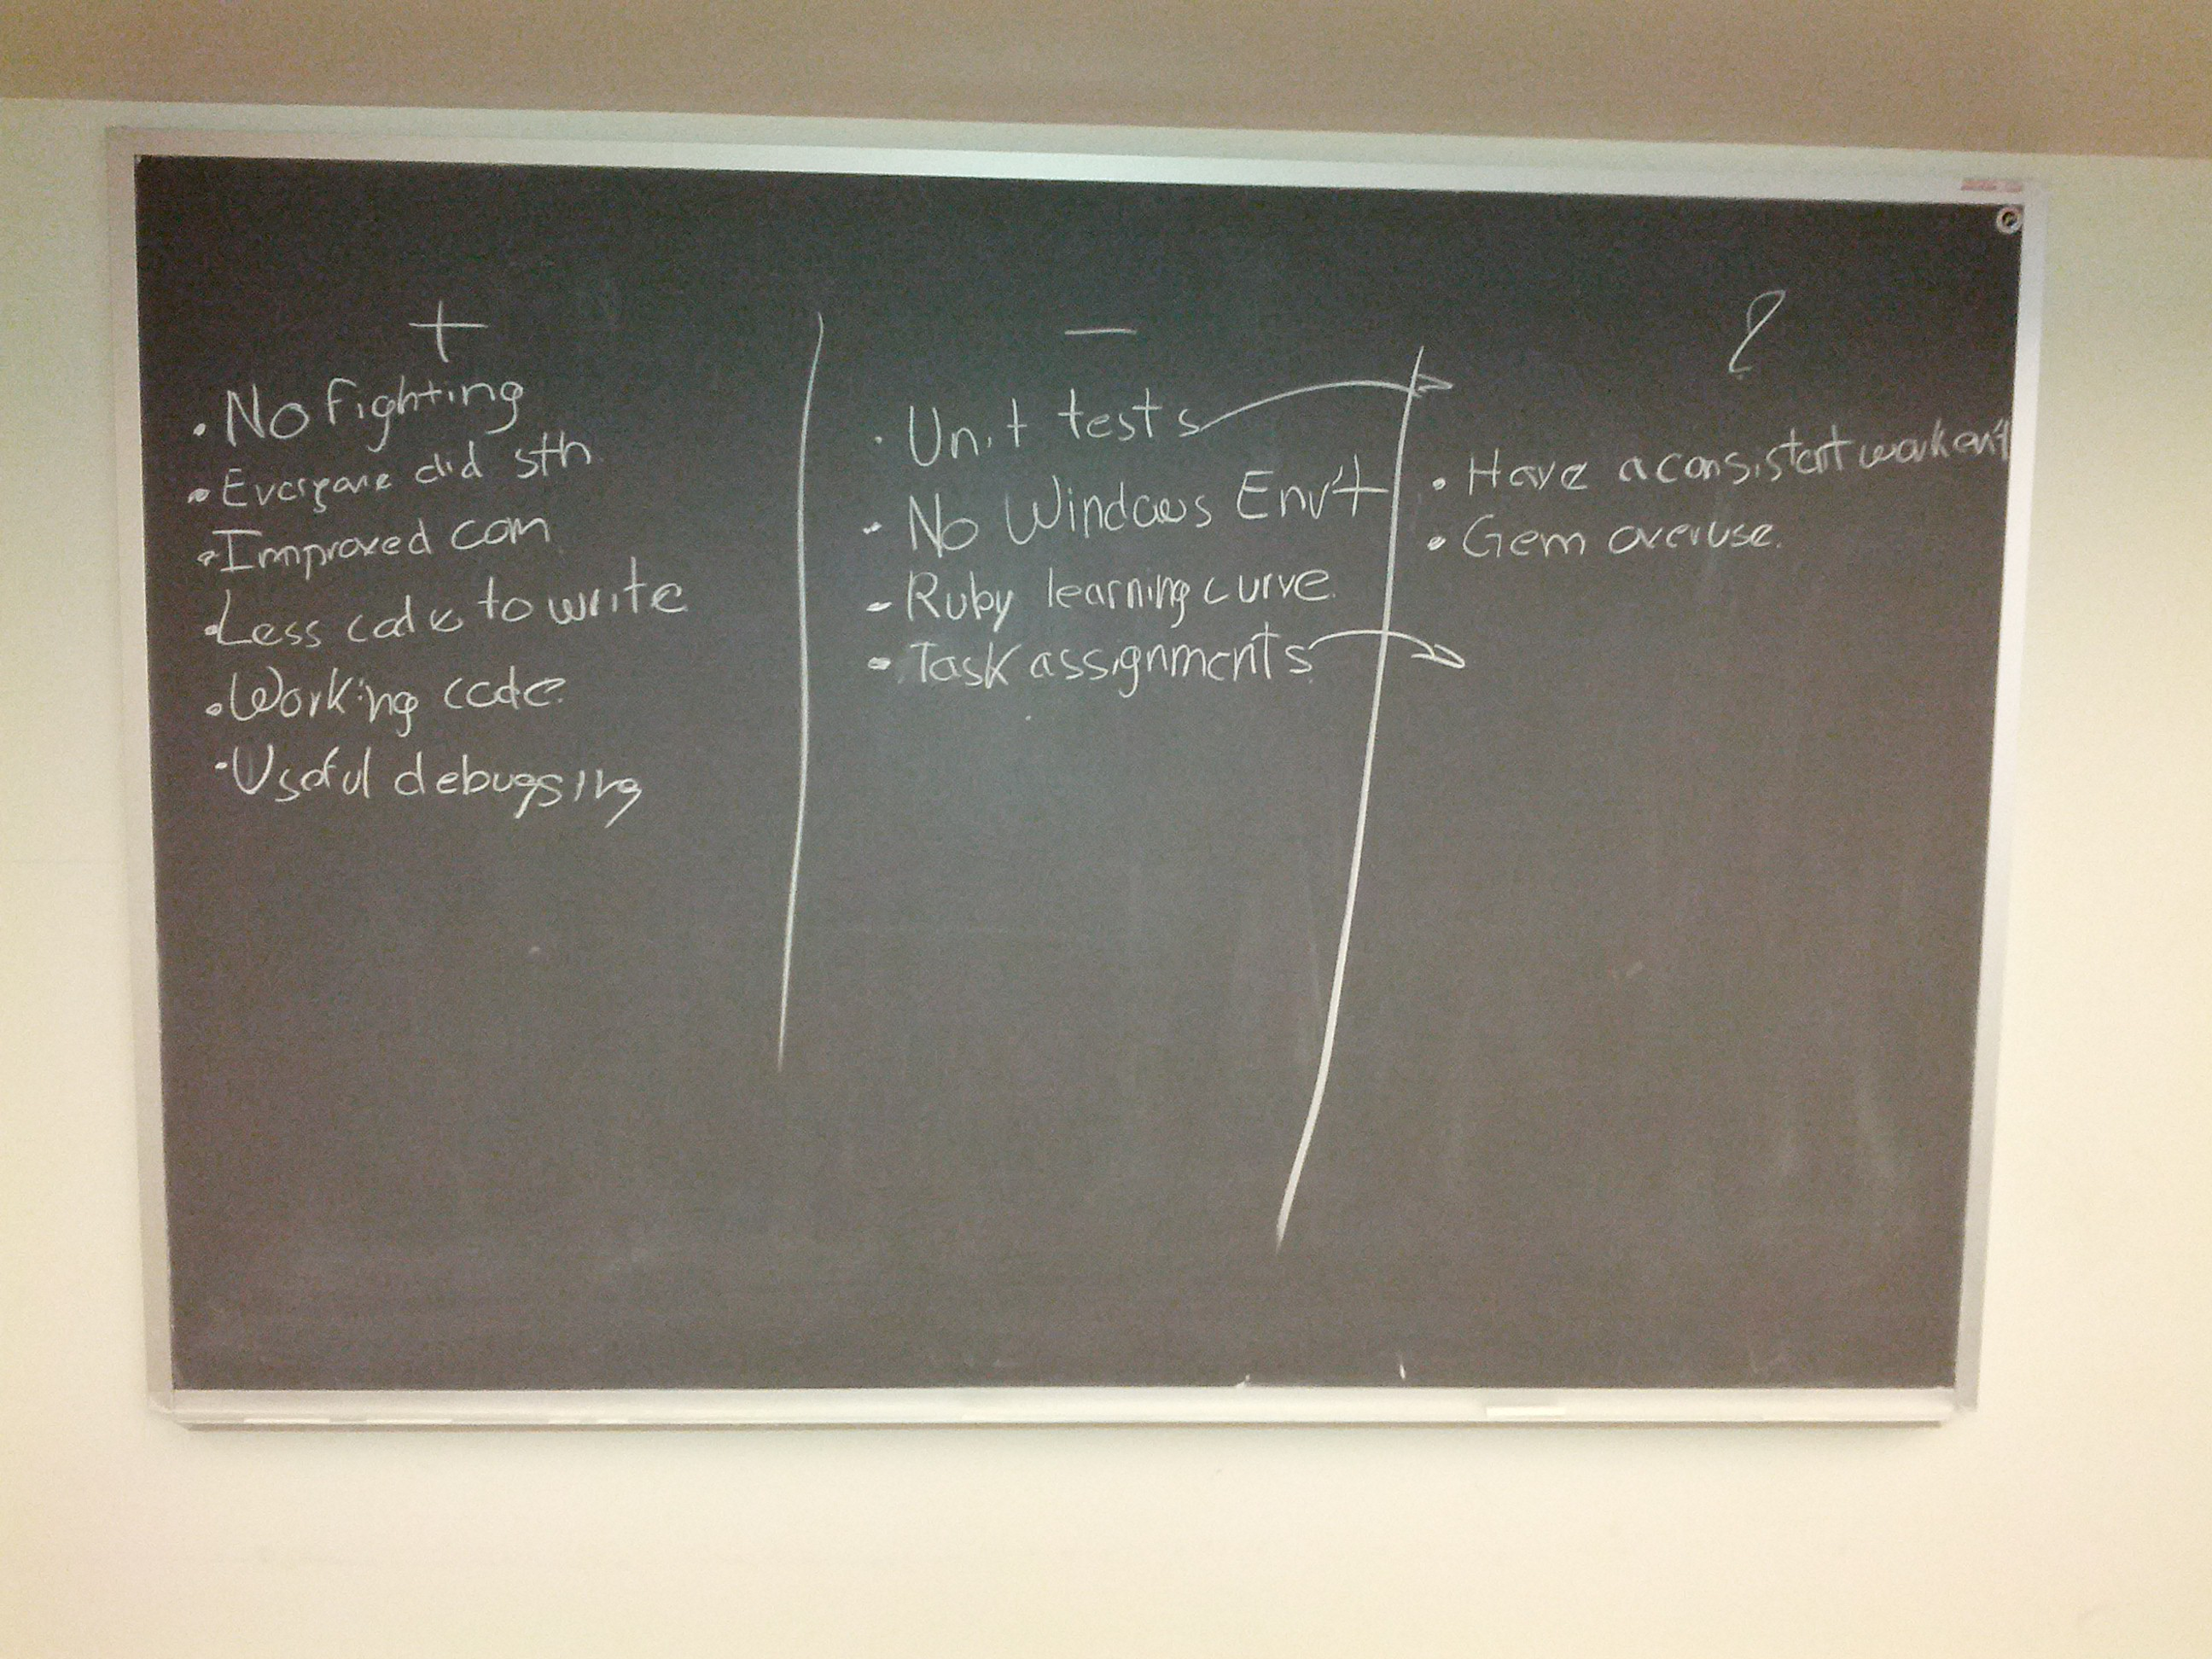
\includegraphics[scale=0.15]{images/retrospective}
	\label{retrospective}
	\caption{Retrospectives}
\end{figure}

\section{Required Changes}

The room availability module (which would have enabled guests to view available rooms without registering) was dropped due to complexity and time constraints. A simple sign-up page was created in lieu of the room availability module. This sign-up page enables users to register and reserve rooms. 

The remaining modules that we had pushed off until iteration 4 would not require changes of the main system to implement. The remaining modules include housekeeping, reporting, and trouble tickets. The housekeeping module would just require adding another user type and restricting the views (which can be done in a very module way since this type of change was already required). The reporting system and trouble ticket system should also not have any impact on the rest of the system except for adding additional tabs to the navigation bar. 

The only change that was requested by our customer was to simplify the invoicing system. The originally proposed invoicing system would have generated a pdf for print-off and would have listed delinquent customer accounts. Instead of this, a simple invoicing page was created which enabled invoice viewing.

\section{Design Evaluation}

\subsection{Design: Coupling, Cohesion, Extensibility}

The hotel management system is built using the Model View Controller (MVC) pattern. This pattern is natively supported by Rails and provides a clean separation between the view and the business logic. The controller layer in the system depends on both the view and the model, the view depends on the model, and the model does not depend on any of the other layers. This resulted in very clean code and a shallow dependency hierarchy. The modules within each layer do not rely on or expose their inner workings to the other modules of the system. Each of the models by convention, provide only a single function and contain closely related methods. All of these combined resulted in a system with low coupling and high cohesion.

\subsection{Testing}

The decision to use ActiveAdmin, and other Gems, to build the hotel manager made us more efficient. By using prebuilt modules we were able to focus on the business logic and leave the more daunting tasks up to the prebuilt modules. ActiveAdmin in particular took care of the user interface and provided the theming and searching support. In addition, we didn't have to write tests for many of the features that we implemented because these gems have already been tested by their developers.

Ruby on Rails is the preeminent prototyping tool as it allowed us to deliver consistent productivity gains. The scaffolding feature allowed for rapid development of modules with very few lines of code, for usability testing and for eliciting customer feedback.

\subsection{Tools}

When new projects are created, three databases are made: a test database, a development database and a production database. This allows for tests to be done without affecting the data in the production database. When a new model is generated in rails, templates for unit and functional tests will be generated automatically in their corresponding folders. 

Git was used as the version control system, which allows developers to check-in code modifications when they're stable enough for other developers to use and test. GitHub was used as the code sharing and publishing service to manage and store revisions of the project. Jenkins was setup for continuous integration, although it was not used since ruby code is dynamically executed and the unit tests all run in short enough time that it would have been more effort than it would have been worth.
\section{Storyboard}

\begin{figure}[!ht]
	\centering
	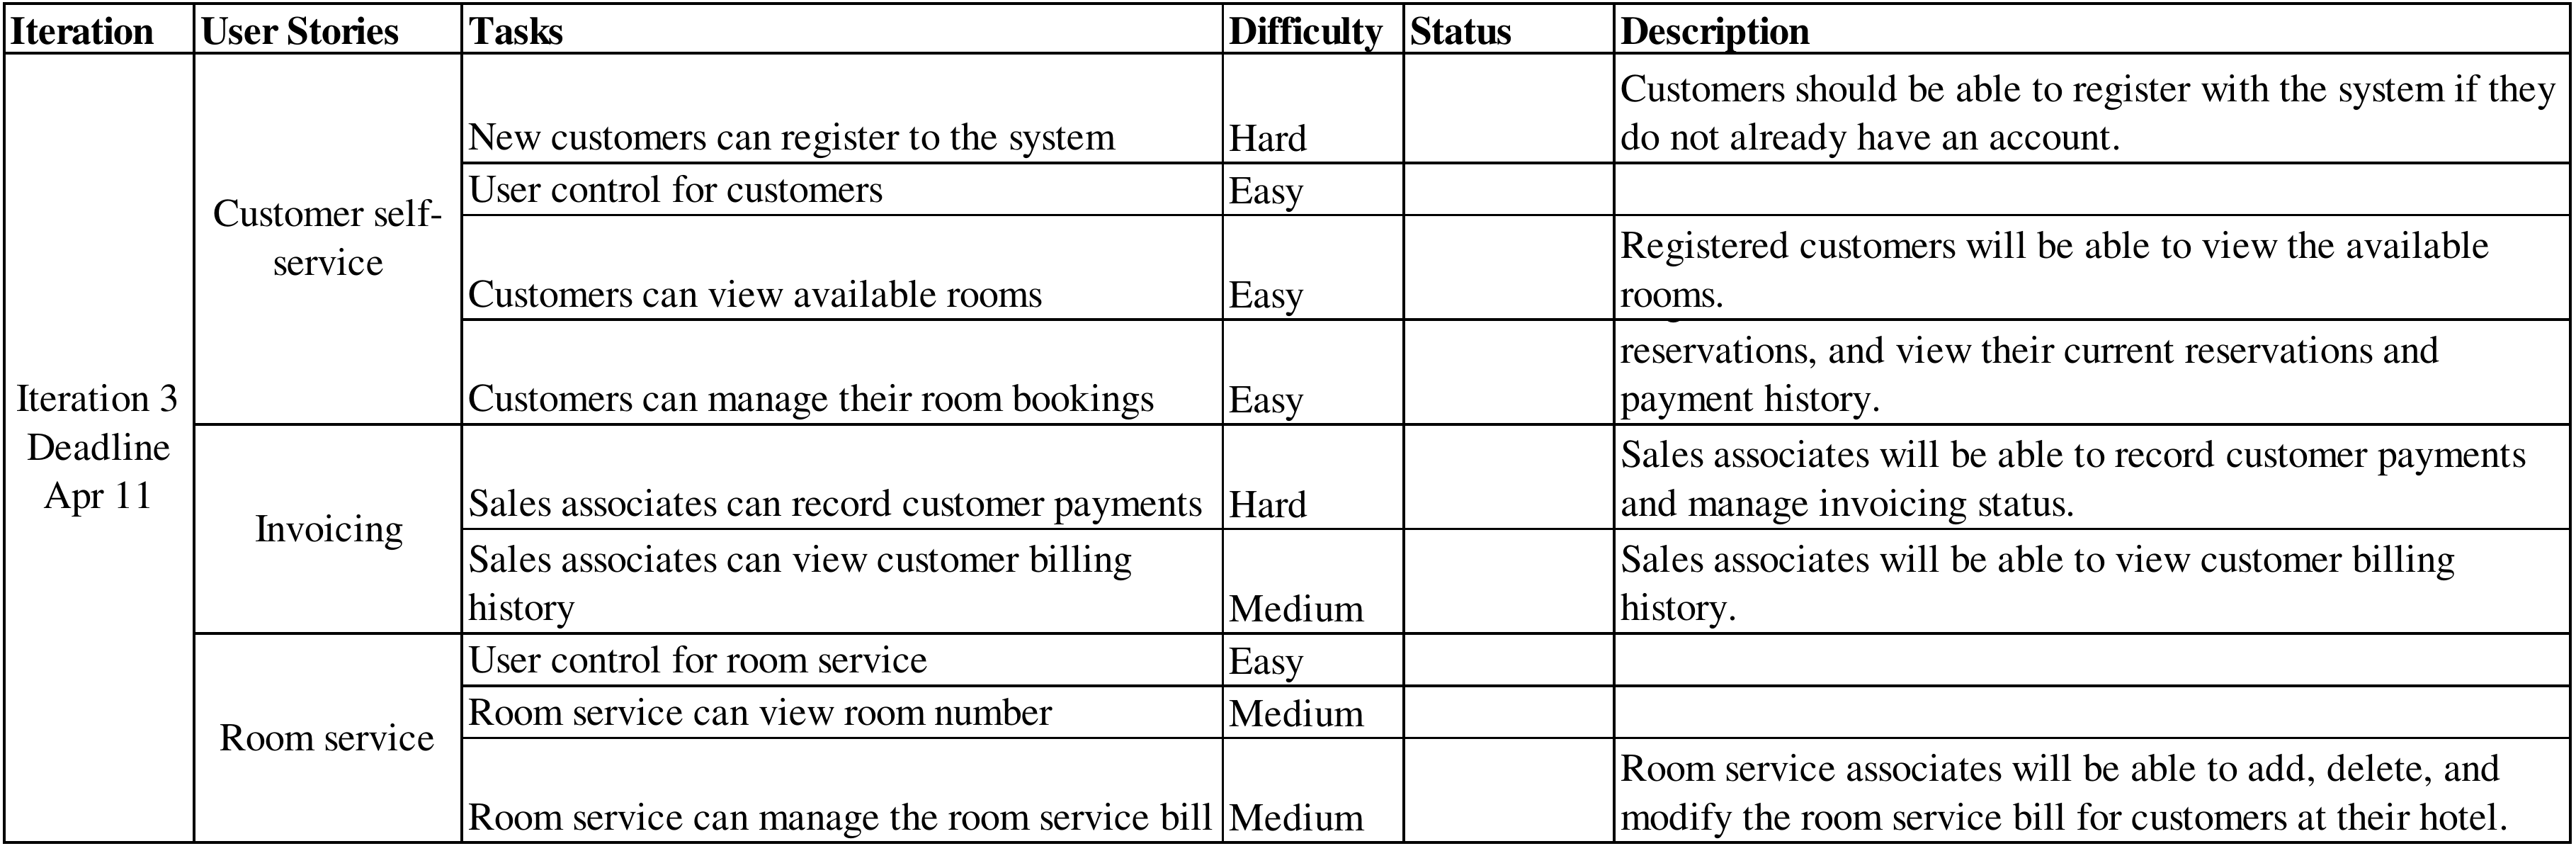
\includegraphics[scale=0.18]{images/storyboard_mar24}
	\caption{Storyboard: March 24}
\end{figure}

\begin{figure}[!ht]
	\centering
	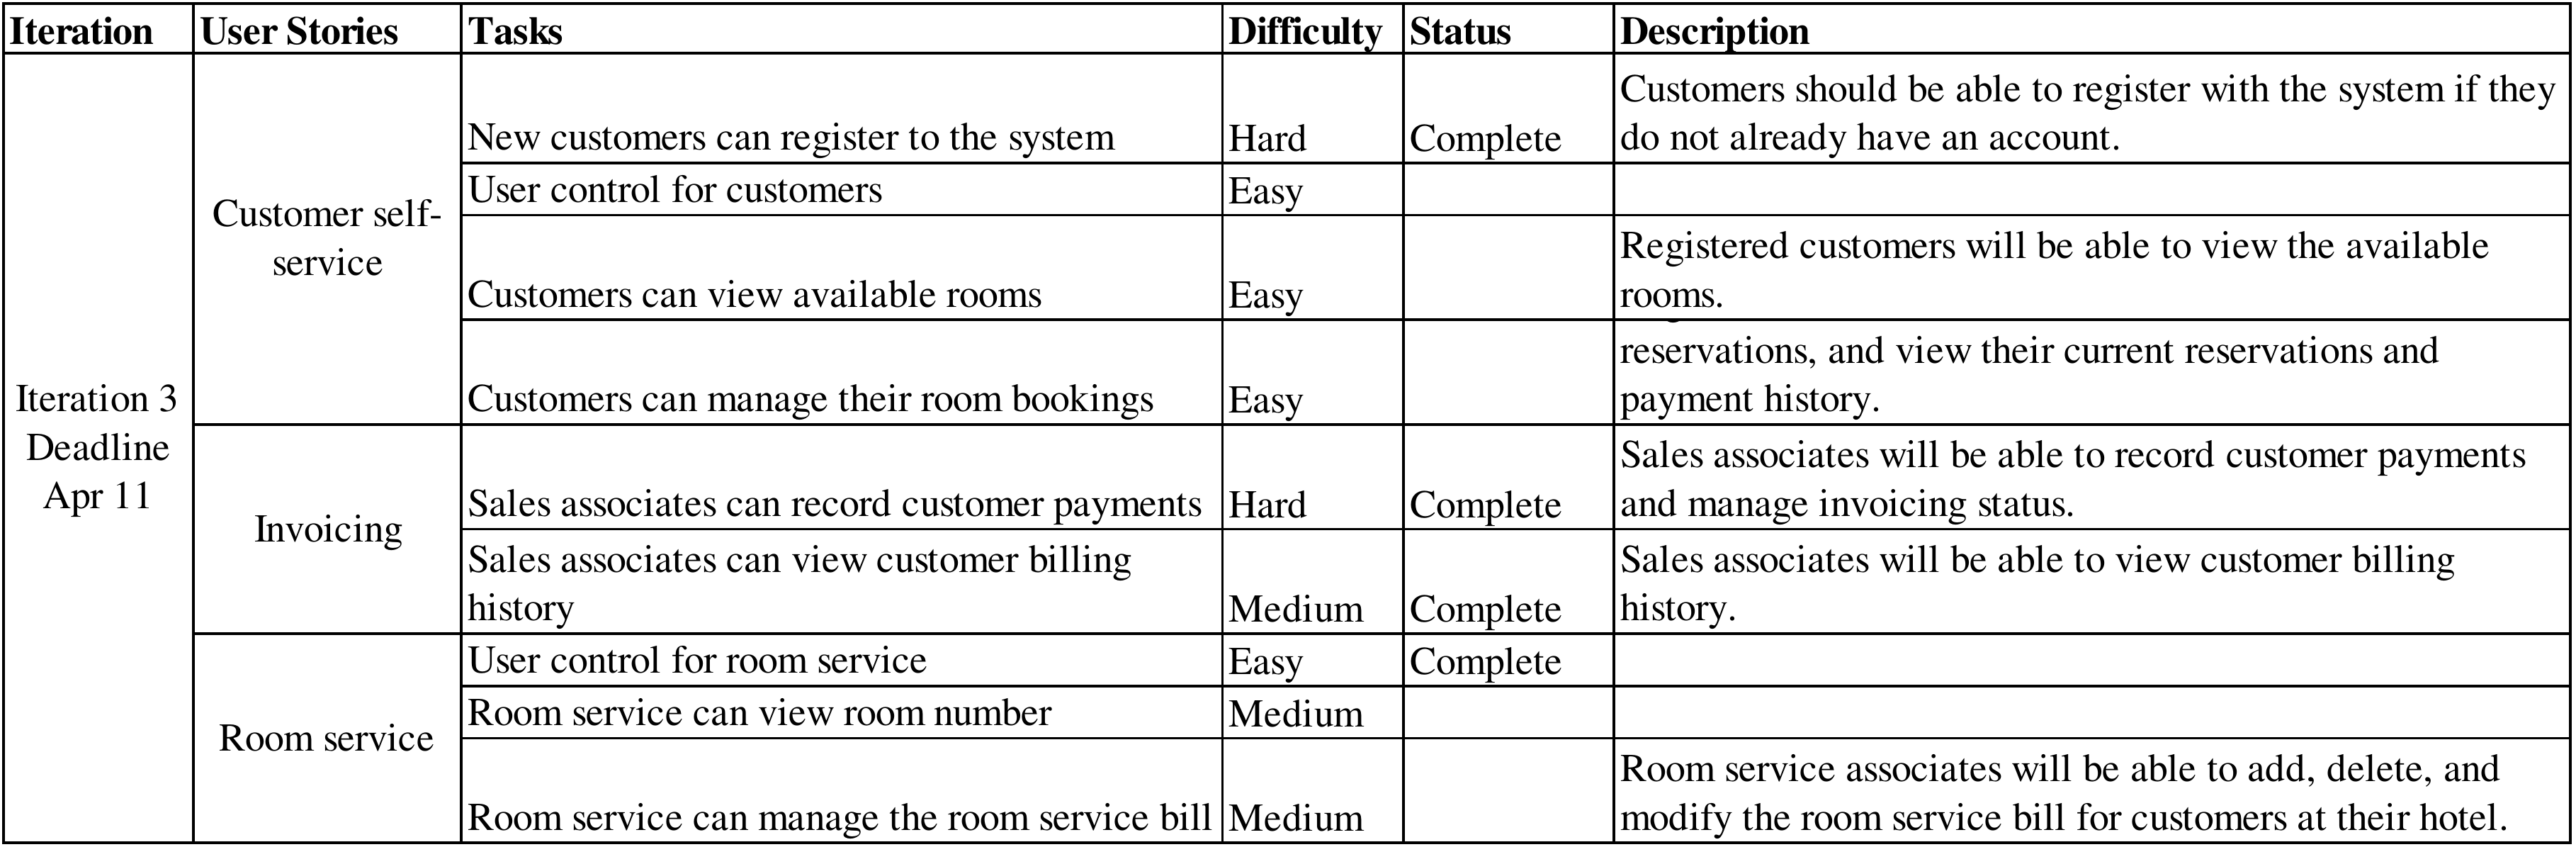
\includegraphics[scale=0.18]{images/storyboard_apr4}
	\caption{Storyboard: April 4}
\end{figure}

\begin{figure}[!ht]
	\centering
	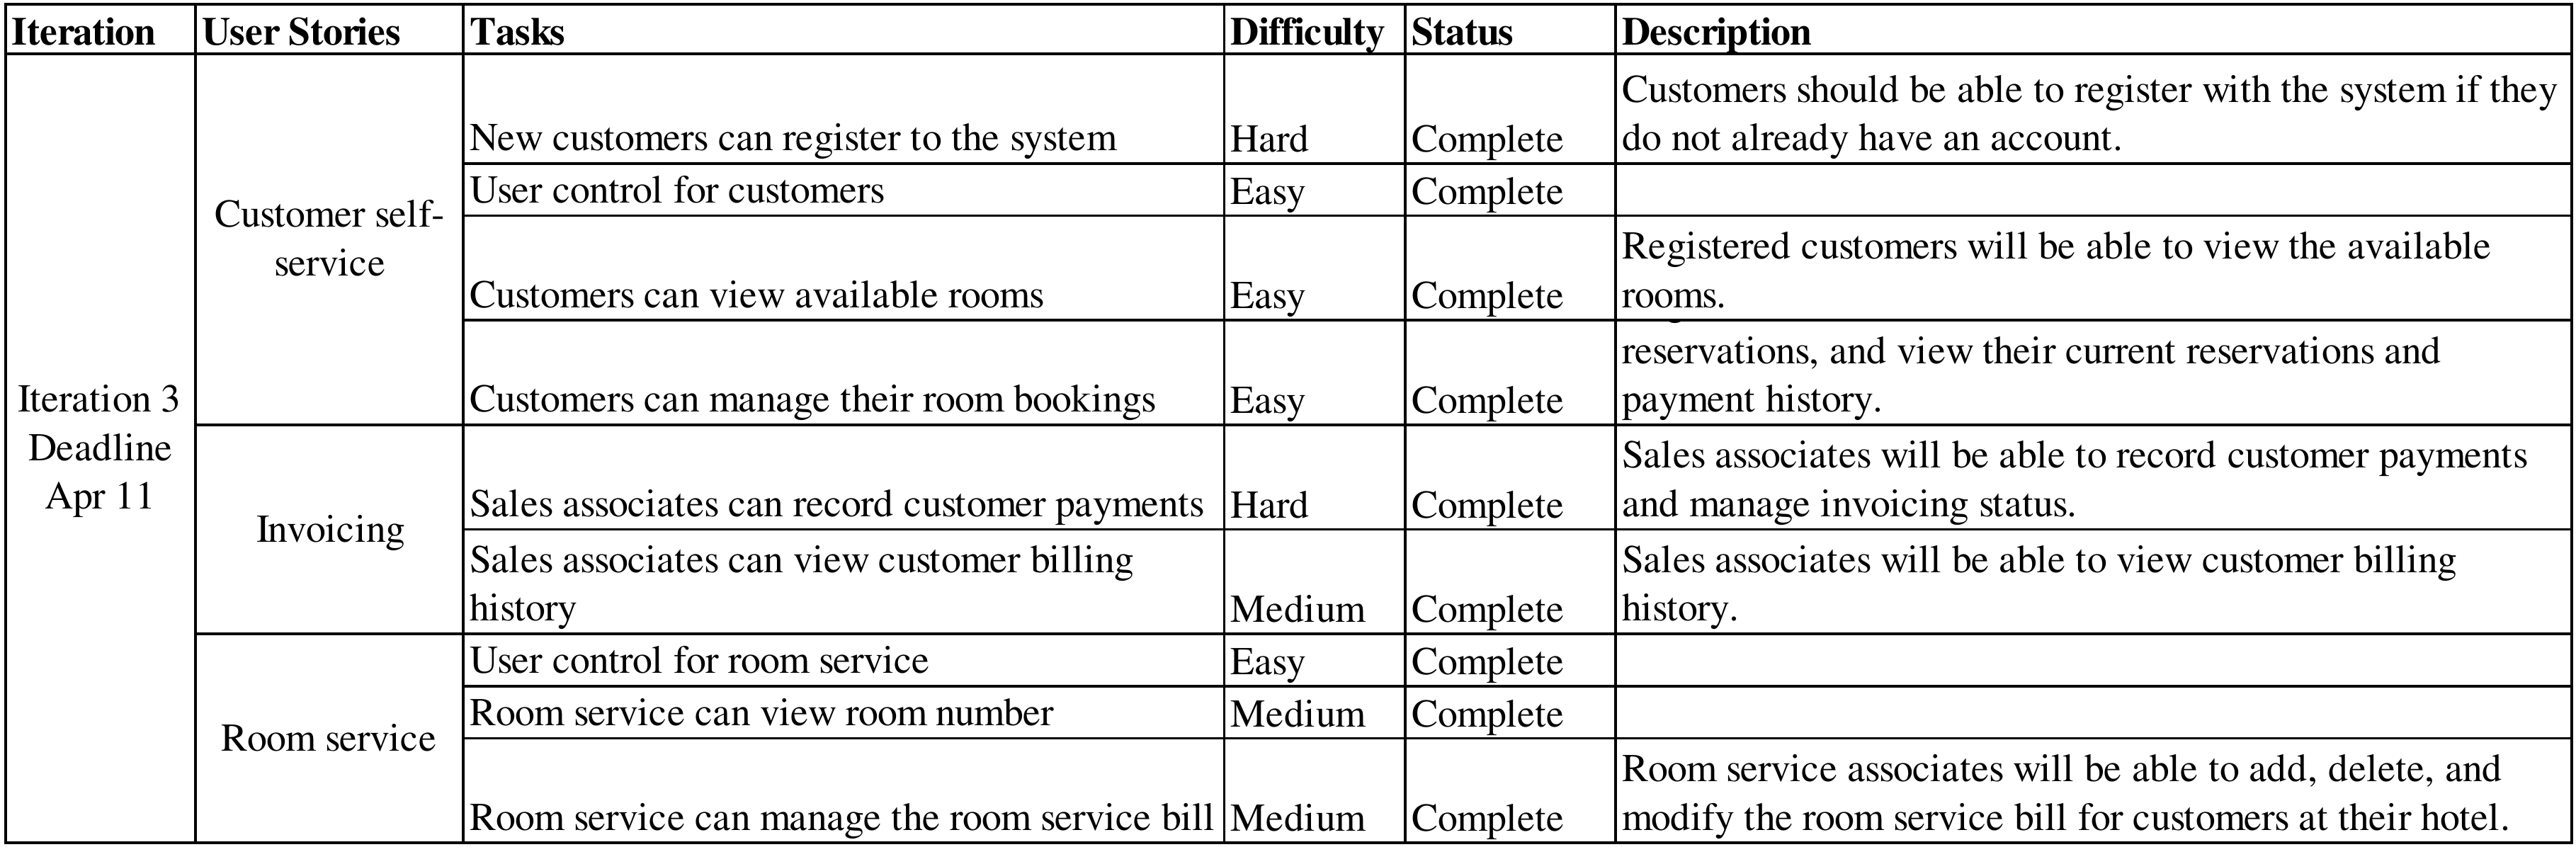
\includegraphics[scale=0.18]{images/storyboard_apr11}
	\caption{Storyboard: April 11}
\end{figure}

\section{Outcomes and Deliverables}

\clearpage
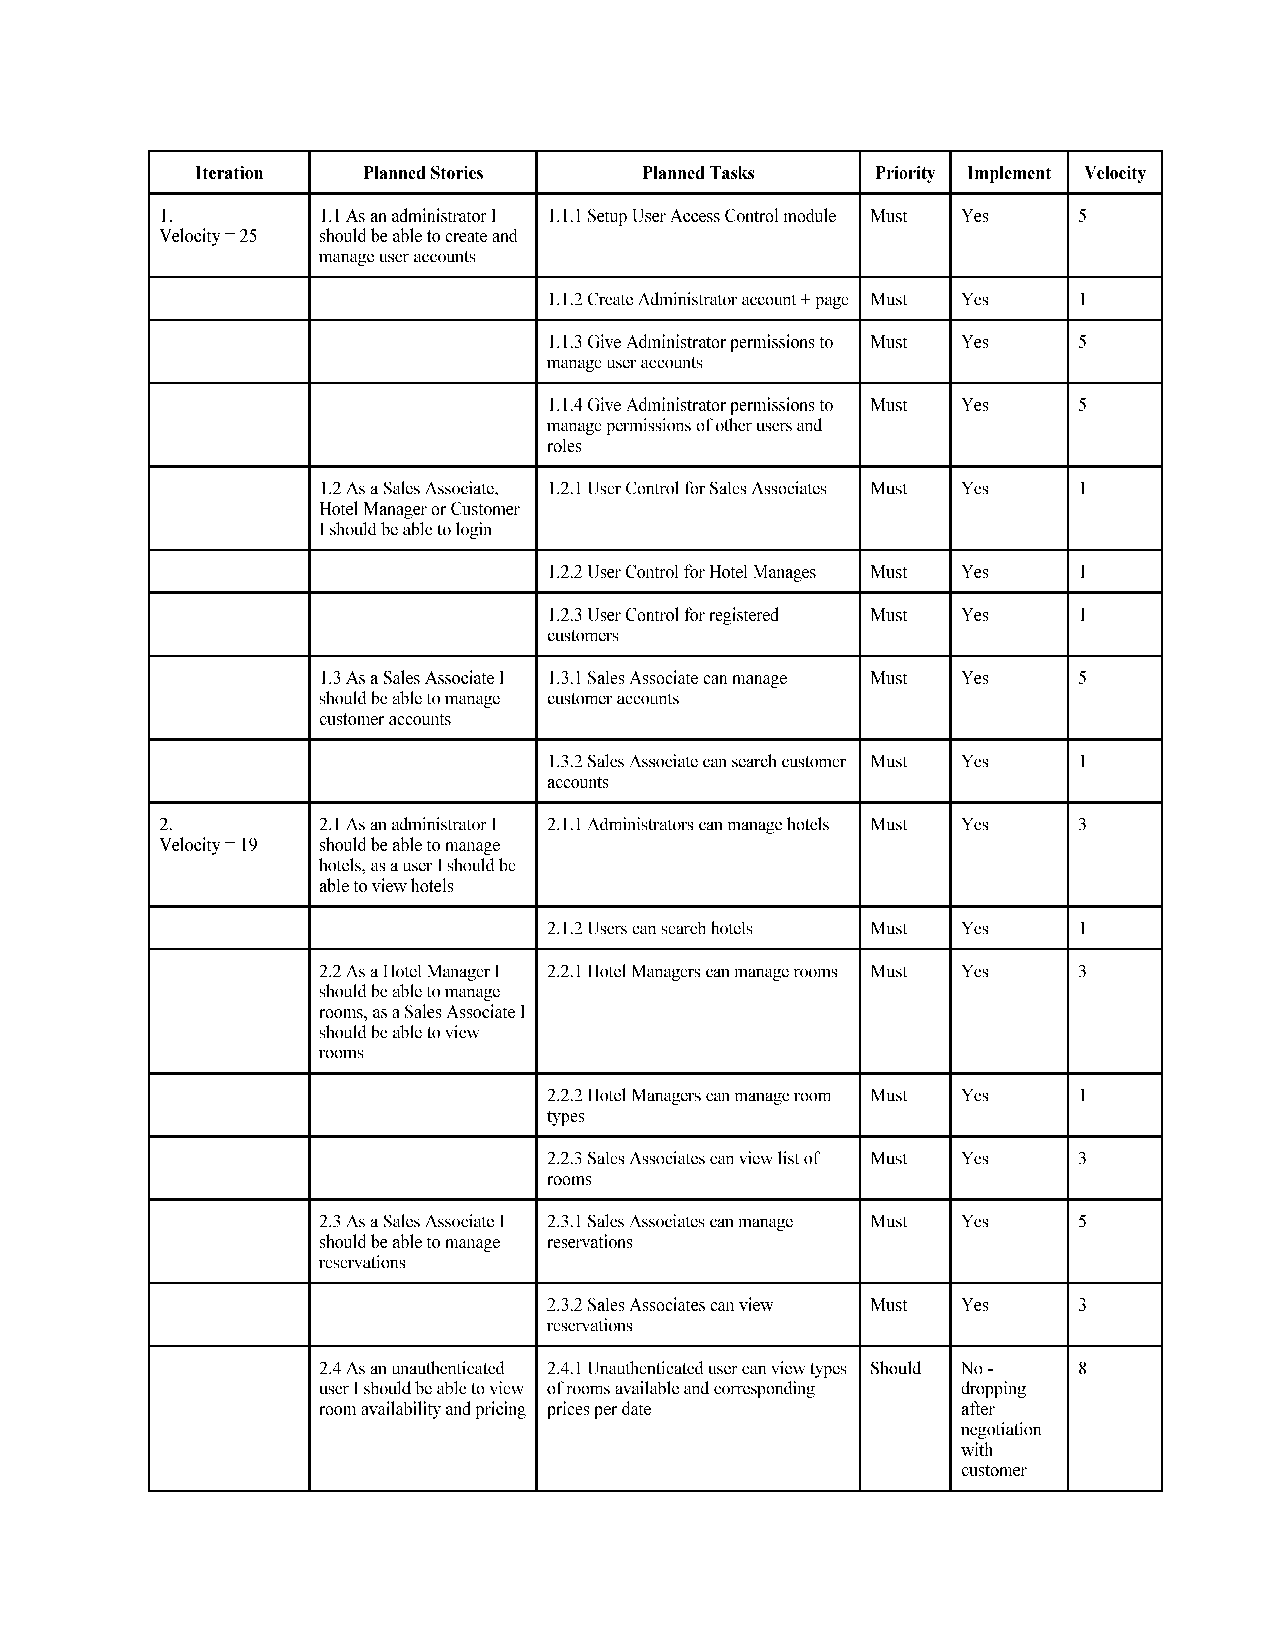
\includepdf[pages={1-}]{include/outcomes_deliverables}

\section{Velocity}

The velocity metric was used to provide a method for measuring the development pace. By tracking velocity, the development team was able to measure the speed that the team was progressing at and more accurately estimate the time to implement the remaining deliverables. Velocity is calculated by estimating the units of work needed to complete all defined tasks in a given iteration by difficulty level. Each task in a project is evaluated in terms of the unit of work. The Iterations are typically three weeks in length and produce tangible deliverables.

Difficulty estimates were computed using the following scale: 1 easy, 3 medium, 5 difficult.

A burn-down chart shows the work remaining, in estimated units, for each iteration. This chart allows the development team to monitor the status of an iteration and estimate the remaining work for that iteration. Figure \ref{burndown} is an example of a burn-down chart that shows the desired velocity for the iteration (red) and the actual velocity (blue). The desired velocity includes the estimates of the tasks that were not completed.

\begin{figure}[!ht]
	\centering
	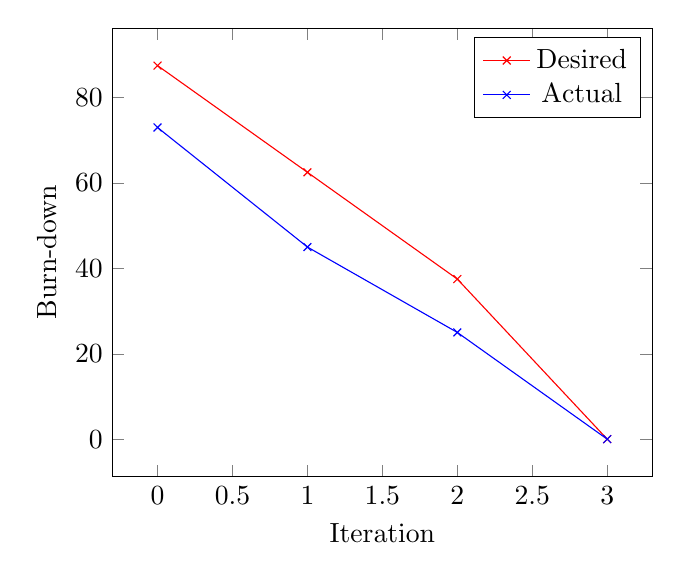
\begin{tikzpicture}
	  \begin{axis}[
			xlabel = Iteration,
			ylabel = Burn-down]
			\addplot[color=red,mark=x] coordinates {
				(0,87.5)
				(1,62.5)
				(2,37.5)
				(3,0)
			};
			\addlegendentry{Desired}
			\addplot[color=blue,mark=x] coordinates {
				(0,73)
				(1,45)
				(2,25)
				(3,0)
			};
			\addlegendentry{Actual}
		\end{axis}
	\end{tikzpicture}
\caption{Burn-down Chart}
\label{burndown}
\end{figure}

\section{Individual Progress}

\begin{table}[!ht]
  \begin{tabular}{|l|p{11cm}|}
    \hline
    \textbf{Team Member} & \textbf{Contributions} \\
    \hline
    Alberto Saavedra & Developed the customer self-service module. Added bootstrap to sign in and sign up forms. \\
    \hline
    Brandon Koepke & Worked with Justin on the report, forced the system to use SSL by default (including certificate generation/etc), fixed the reservation date range validation, fixed the reservation naming, setup the demo server. \\
    \hline
    Garrick Van Der Lee & Developed the Room Service module and fixed a few minor bugs with older code. Helped out a bit with invoice. \\
    \hline
    Julia Paredes & Developed the invoice module. Added check-in check-out functionality. Helped out with some bugs. \\
    \hline
    Justin Milanovic & Worked with Brandon to complete the outcomes and deliverables report. Also worked with Alberto to complete the guest user system. \\
    \hline
    Tyler Gibb & Worked on the Room Service model, adjusted the price validator, and helped out with various debugging and syntax errors. \\
    \hline
  \end{tabular}
	\caption{Individual Progress}
\end{table}

\end{document}
